\documentclass{classrep}
\usepackage[utf8]{inputenc}
\usepackage{color}
\usepackage[utf8]{inputenc}
\usepackage{amssymb}
\usepackage{polski}
\usepackage[polish]{babel}
\usepackage{amsmath}
\usepackage{amsfonts}
\usepackage{lastpage}
\usepackage{fontawesome}
\usepackage{graphicx}
\usepackage{float}
\usepackage{geometry}
\usepackage{caption}
\usepackage{subcaption}
\captionsetup{compatibility=false}

\DeclareUnicodeCharacter{00A0}{~}

\studycycle{Informatyka, studia dzienne, inż I st.}
\coursesemester{V}

\coursename{Sztuczna inteligencja i systemy ekspertowe}
\courseyear{2018/2019}

\courseteacher{Przemysław Nowak}
\coursegroup{Czwartek, 12:00}

\author{
  \studentinfo{Patryk Lisik}{210254} \and
  \studentinfo{Adam Sadowski}{210310}
}

\title{Zadanie 1: Piętnastka}

\def \hfillx {\hspace*{-\textwidth} \hfill}

\begin{document}
\maketitle


\section{Cel}
Implementacja kilku algorytmów rozwiązywania gry logicznej "Piętnastki" i analiza ich efektywności.

\section{Wprowadzenie}
\subsection{Piętnastka}
\begin{table}[h!]
    \begin{minipage}{0.5\textwidth}
        \centering
        \begin{tabular}{|l|l|l|l|}
            \hline
            1 & 2 & 3 & 4 \\ \hline
            5 & 6 & 7 & 8 \\ \hline
            9 & 10 & 11 & 12 \\ \hline
            13 & 14 & 15 &  \\ \hline
            \end{tabular}
        \caption{Rozwiązana piętnastka}
        \label{tab:solved}
    \end{minipage}
    \hfillx
    \begin{minipage}{0.5\textwidth}
        \centering
        \begin{tabular}{|l|l|l|l|}
            \hline
            1 & 2 & 3 & 4 \\ \hline
            5 & 6 & 7 & 8 \\ \hline
            9 & 10 & 11 & 12 \\ \hline
            13 & 14 &  & 15 \\ \hline
            \end{tabular}
        \caption{Układ wymagający jednego ruchu}
    \end{minipage}
\end{table}

Piętnastka jest grą logiczną wymyśloną pod koniec XIX wieku.
Jej nazwa pochodzi od piętnastu ponumerowanych 1--15, które trzeba ułożyć tak jak w tablicy \ref{tab:solved}.

Stan końcowego musi musi zostać osiągnięty jedynie poprzez ruchy pustego pola w obrębie macierzy $4\times 4$. 
Jeśli puste pole znajduje sie przy krawędzi niektóre ruchy mogą nie być dozwolone.
W dalszej części ruchy będą oznaczane.
\begin{itemize}
    \item L -- (ang. left) w lewo
    \item R -- (ang. right) w prawo
    \item D -- (ang. down) w dół
    \item U -- (ang. up) w górę
\end{itemize}

\subsection{Grafy}
Grafem nazywamy strukturę danych modelującą zbiór wierzchołków i połączeń między nimi.
\subsubsection{Reprezenatacja}
\begin{figure}[h]
    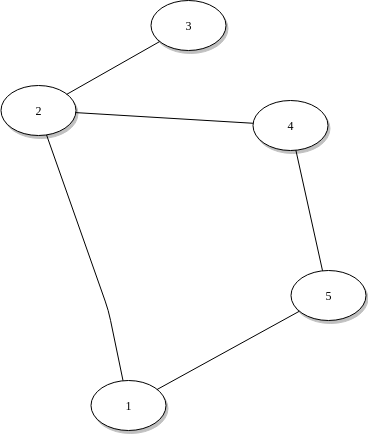
\includegraphics[scale = 0.4]{graf.png}
    \caption{Przykładowy graf}
\end{figure}
\paragraph{Macierz sąsiedztwa}
\begin{table}[h!]
    \begin{tabular}{|l|lllll}
    \hline
     & \multicolumn{1}{l|}{1} & \multicolumn{1}{l|}{2} & \multicolumn{1}{l|}{3} & \multicolumn{1}{l|}{4} & \multicolumn{1}{l|}{5} \\ \hline
    1 & 0 & 1 & 0 & 0 & 0 \\ \cline{1-1}
    2 & 1 & 0 & 1 & 1 & 1 \\ \cline{1-1}
    3 & 0 & 1 & 0 & 0 & 0 \\ \cline{1-1}
    4 & 0 & 1 & 0 & 0 & 1 \\ \cline{1-1}
    5 & 1 & 0 & 0 & 1 & 0 \\ \cline{1-1}
    \end{tabular}
    \caption{Przykładowa macierz sąsiedztwa}
    \label{my-label}
    \end{table}

 \paragraph{Lista sąsiedztwa}

\subsubsection{Metody przeszukiwania}
\begin{description}
    \item [DFS] Depth first search -- przeszukiwanie w głąb
    \item [BFS] Breath first search -- przeszukiwanie w szerz
    \item [A*] Przeszukiwanie oparte o heurystykę
    \begin{description}
        \item [Manhattan]
        \item [Hamminga]
    \end{description}
\end{description}

\subsubsection{Pozostałe pojęcia}
\begin{description}
    \item [Cykl]
    \item [Droga]
    \item 
\end{description}

\section{Opis implementacji}
{\color{blue}
Należy tu zamieścić krótki i zwięzły opis zaprojektowanych klas oraz powiązań
między nimi. Powinien się tu również znaleźć diagram UML (diagram klas)
prezentujący najistotniejsze elementy stworzonej aplikacji. Należy także podać,
w jakim języku programowania została stworzona aplikacja.}

\section{Materiały i metody}
{\color{blue}
W tym miejscu należy opisać, jak przeprowadzone zostały wszystkie badania,
których wyniki i dyskusja zamieszczane są w dalszych sekcjach. Opis ten
powinien być na tyle dokładny, aby osoba czytająca go potrafiła wszystkie
przeprowadzone badania samodzielnie powtórzyć w celu zweryfikowania ich
poprawności. Przy opisie należy odwoływać się i stosować do
opisanych w sekcji drugiej wzorów i oznaczeń, a także w jasny sposób opisać
cel konkretnego testu. Najlepiej byłoby wyraźnie wyszczególnić (ponumerować)
poszczególne eksperymenty tak, aby łatwo było się do nich odwoływać dalej.}

\section{Wyniki}
\newgeometry{left=1cm,right=0.1cm,bottom=4cm}
\begin{figure}[H]
    \centering
    \begin{subfigure}[t]{0.45\textwidth}
        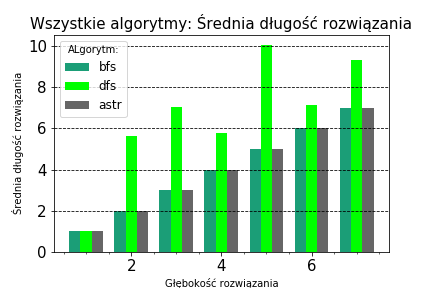
\includegraphics[width=\textwidth]{charts/ALL_path_length.png}
        \caption{Średnia długość rozwiązania}
        \label{ALL:path_length}
    \end{subfigure}
    ~ %add desired spacing between images, e. g. ~, \quad, \qquad, \hfill etc. 
      %(or a blank line to force the subfigure onto a new line)
    \begin{subfigure}[t]{0.45\textwidth}
        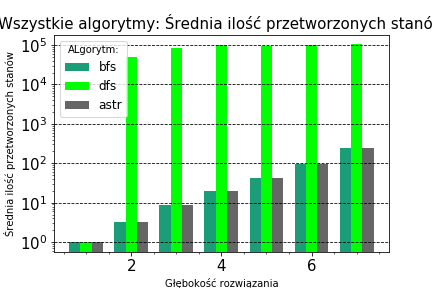
\includegraphics[width=\textwidth]{charts/ALL_processed.png}
        \caption{Średnia ilość przetworzonych stanów}
        \label{ALL:processed}
    \end{subfigure}
    \qquad
    ~ %add desired spacing between images, e. g. ~, \quad, \qquad, \hfill etc. 
    %(or a blank line to force the subfigure onto a new line)
    \begin{subfigure}[t]{0.45\textwidth}
        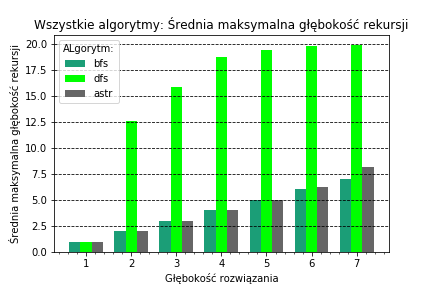
\includegraphics[width=\textwidth]{charts/ALL_recursed.png}
        \caption{Średnia maksymalna głębokość rekursji}
        \label{ALL:rescursed}
    \end{subfigure}
    \begin{subfigure}[t]{0.45\textwidth}
        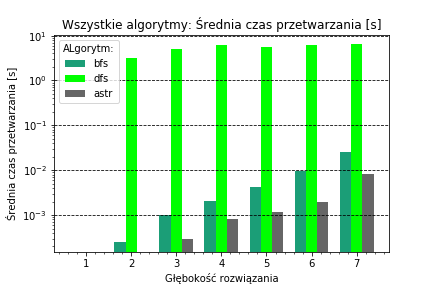
\includegraphics[width=\textwidth]{charts/ALL_time.png}
        \caption{Średni czas przetwarzania}
        \label{ALL:time}
    \end{subfigure}
    \begin{subfigure}[t]{0.45\textwidth}
        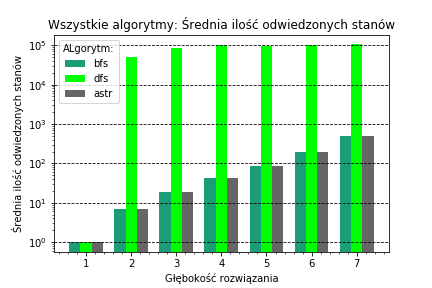
\includegraphics[width=\textwidth]{charts/ALL_visited.png}
        \caption{Średnia ilość odwiedzonych stanów}
        \label{ALL:visited}
    \end{subfigure}
    \caption{Porównanie wszystkich metod przeszukiwania}\label{col:all}
\end{figure}

\begin{figure}[H]
    \centering
    \begin{subfigure}[t]{0.45\textwidth}
        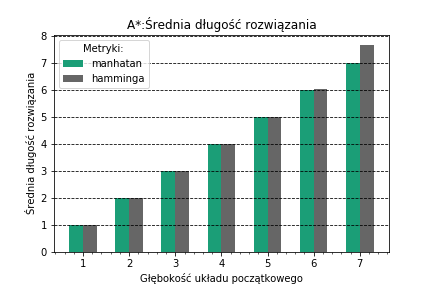
\includegraphics[width=\textwidth]{charts/ASTR_path_length.png}
        \caption{Średnia długość rozwiązania}
        \label{ASTR:path_length}
    \end{subfigure}
    ~ %add desired spacing between images, e. g. ~, \quad, \qquad, \hfill etc. 
      %(or a blank line to force the subfigure onto a new line)
    \begin{subfigure}[t]{0.45\textwidth}
        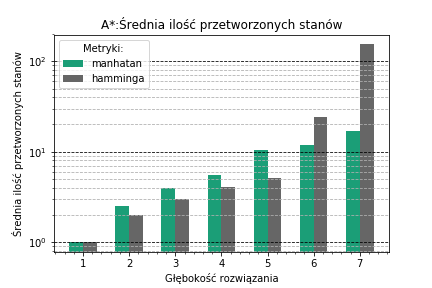
\includegraphics[width=\textwidth]{charts/ASTR_processed.png}
        \caption{Średnia ilość przetworzonych stanów}
        \label{ASTR:processed}
    \end{subfigure}
    \qquad
    ~ %add desired spacing between images, e. g. ~, \quad, \qquad, \hfill etc. 
    %(or a blank line to force the subfigure onto a new line)
    \begin{subfigure}[t]{0.45\textwidth}
        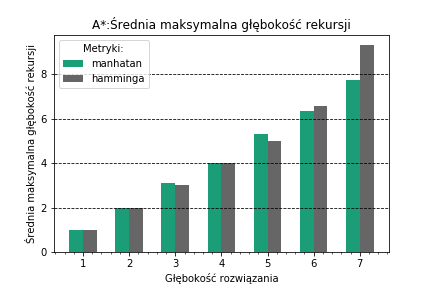
\includegraphics[width=\textwidth]{charts/ASTR_recursed.png}
        \caption{Średnia maksymalna głębokość rekursji}
        \label{ASTR:rescursed}
    \end{subfigure}
    \begin{subfigure}[t]{0.45\textwidth}
        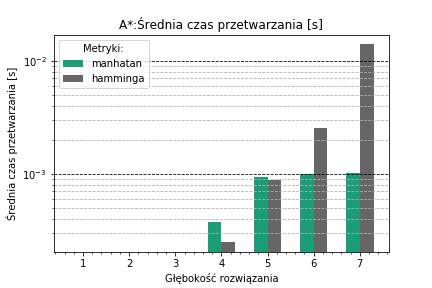
\includegraphics[width=\textwidth]{charts/ASTR_time.png}
        \caption{Średni czas przetwarzania}
        \label{ASTR:time}
    \end{subfigure}
    \begin{subfigure}[t]{0.45\textwidth}
        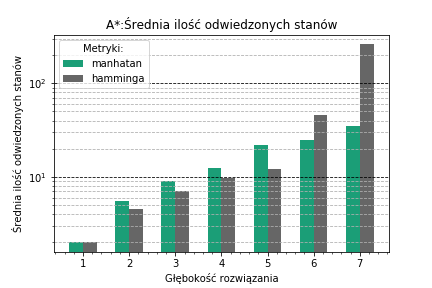
\includegraphics[width=\textwidth]{charts/ASTR_visited.png}
        \caption{Średnia ilość odwiedzonych stanów}
        \label{ASTR:visited}
    \end{subfigure}
    \caption{Porównanie wszystkich metod przeszukiwania}\label{coll:astr}
\end{figure}

\begin{figure}[H]
    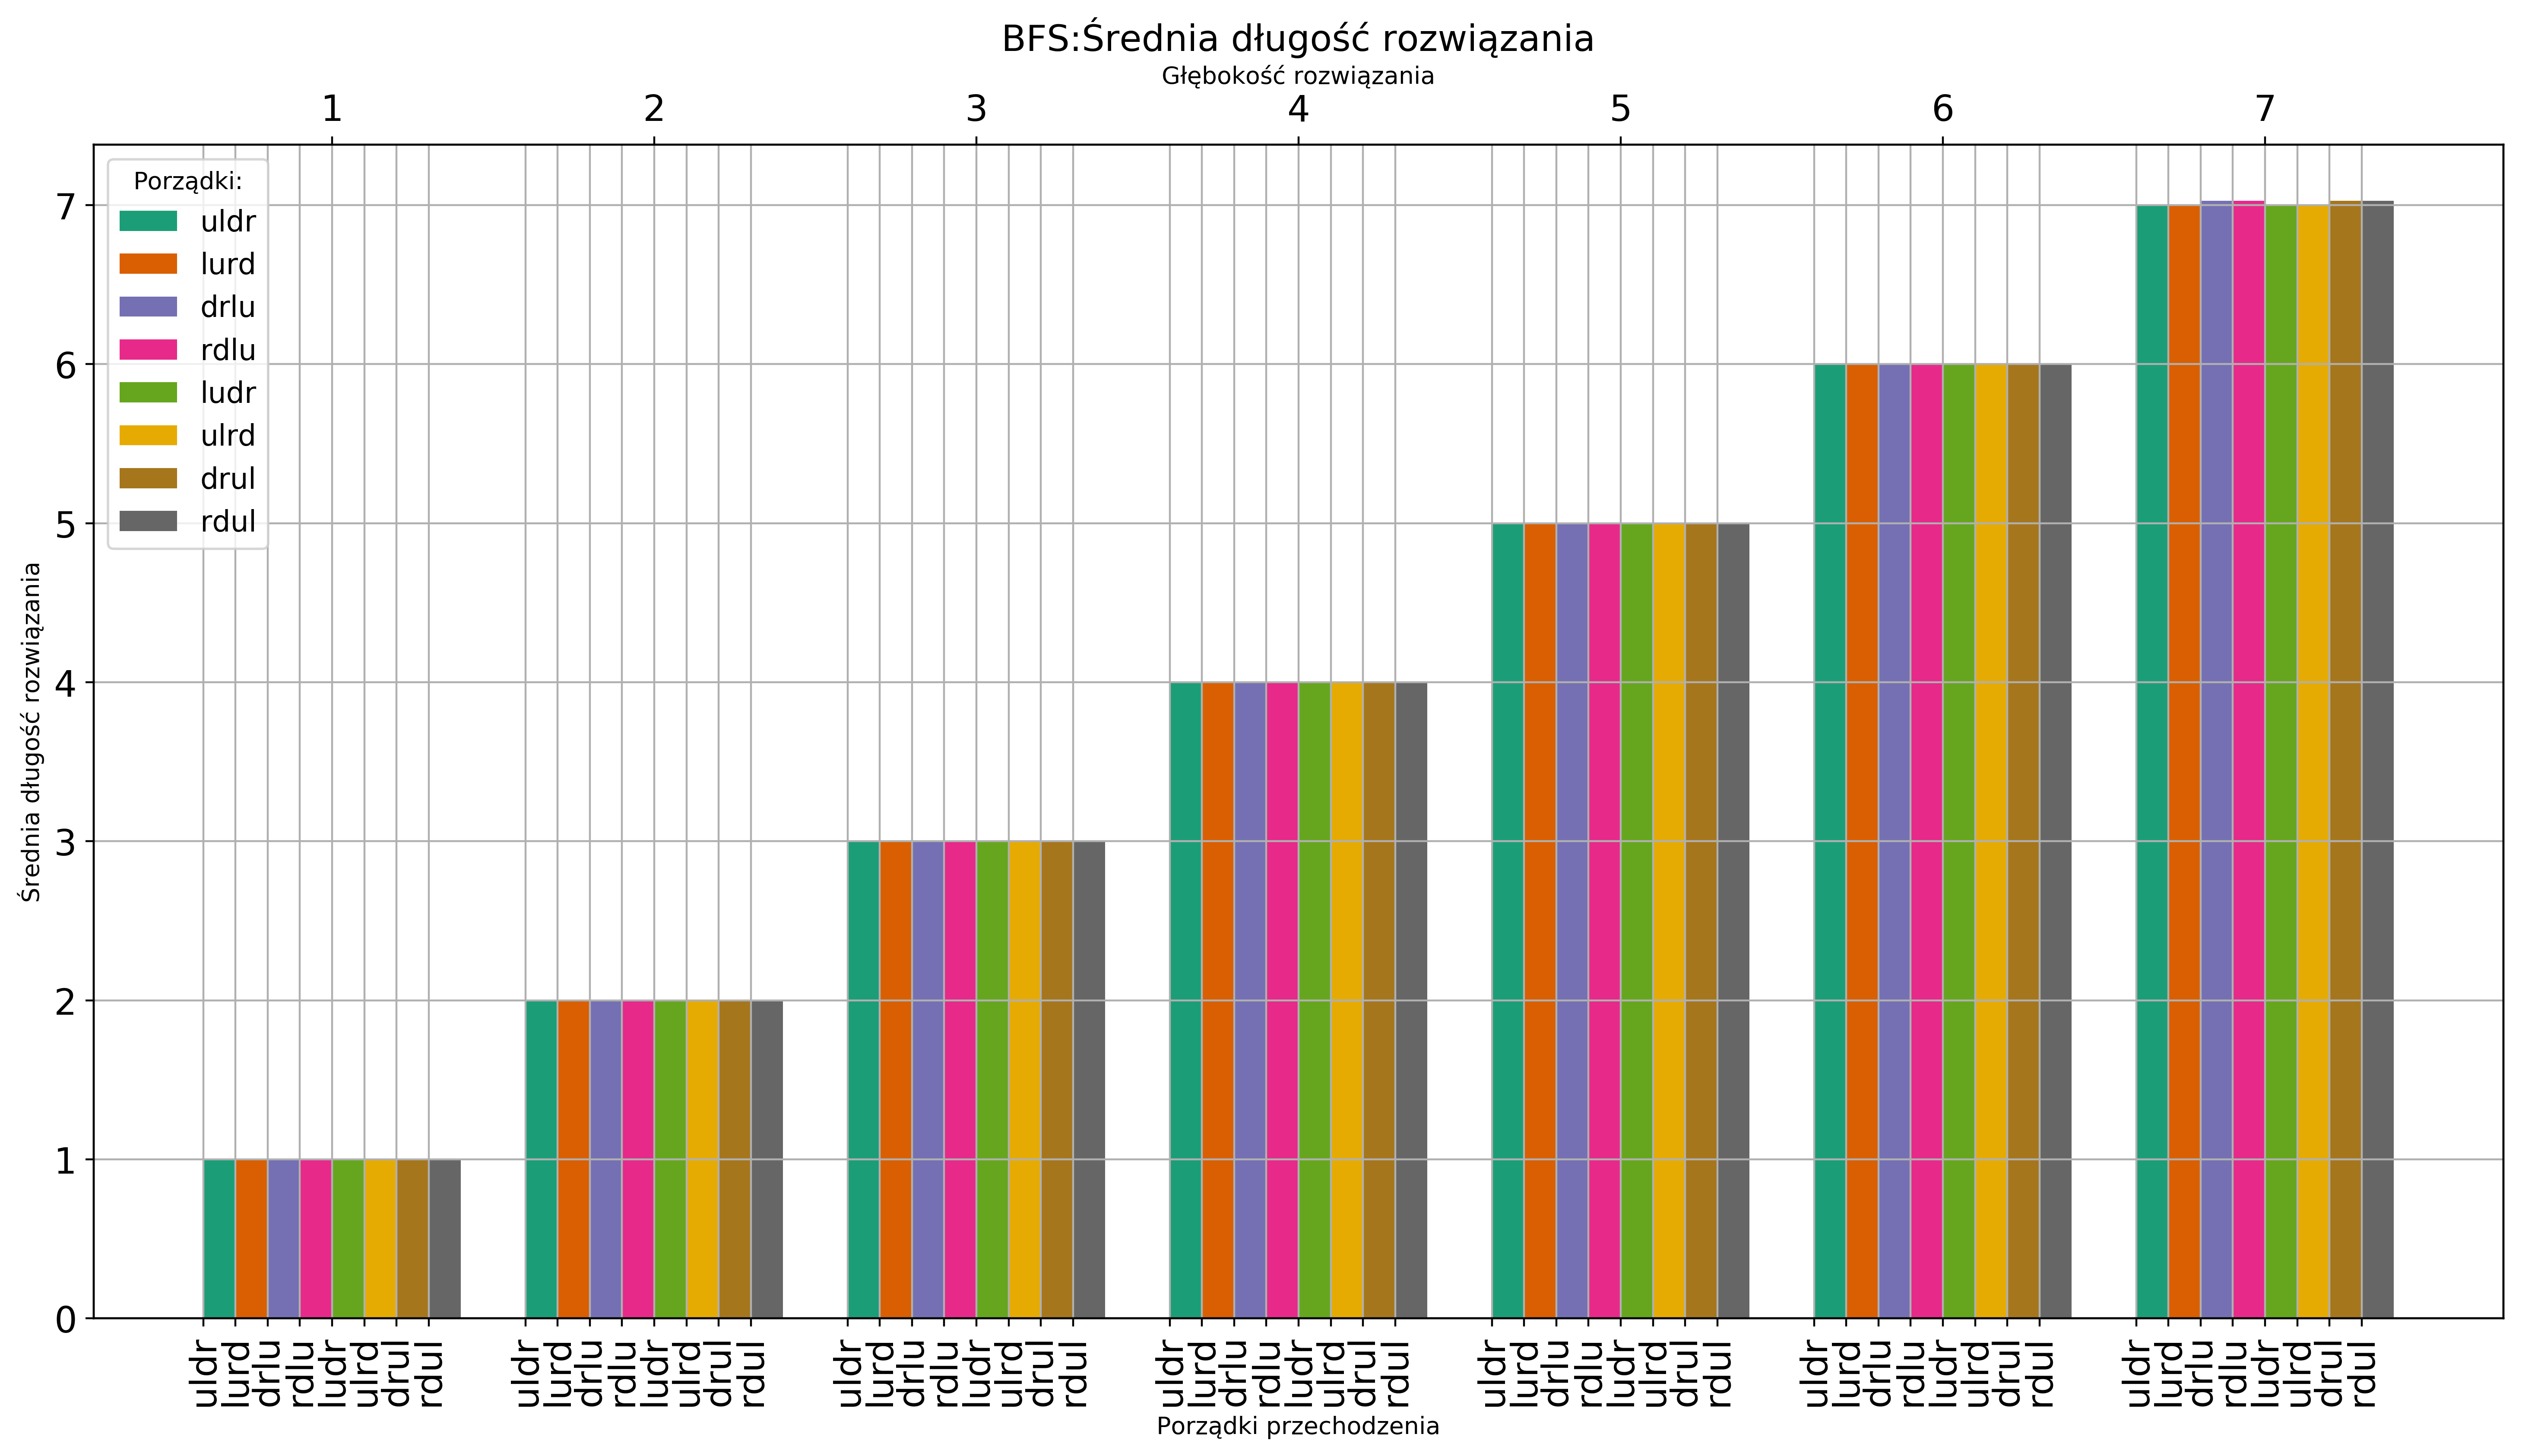
\includegraphics[width=\textwidth]{charts/BFS_path_length.png}
    \caption{BFS -- Średnia długość rozwiązania}
    \label{BFS:path_length}
    \vspace{0.2cm}
    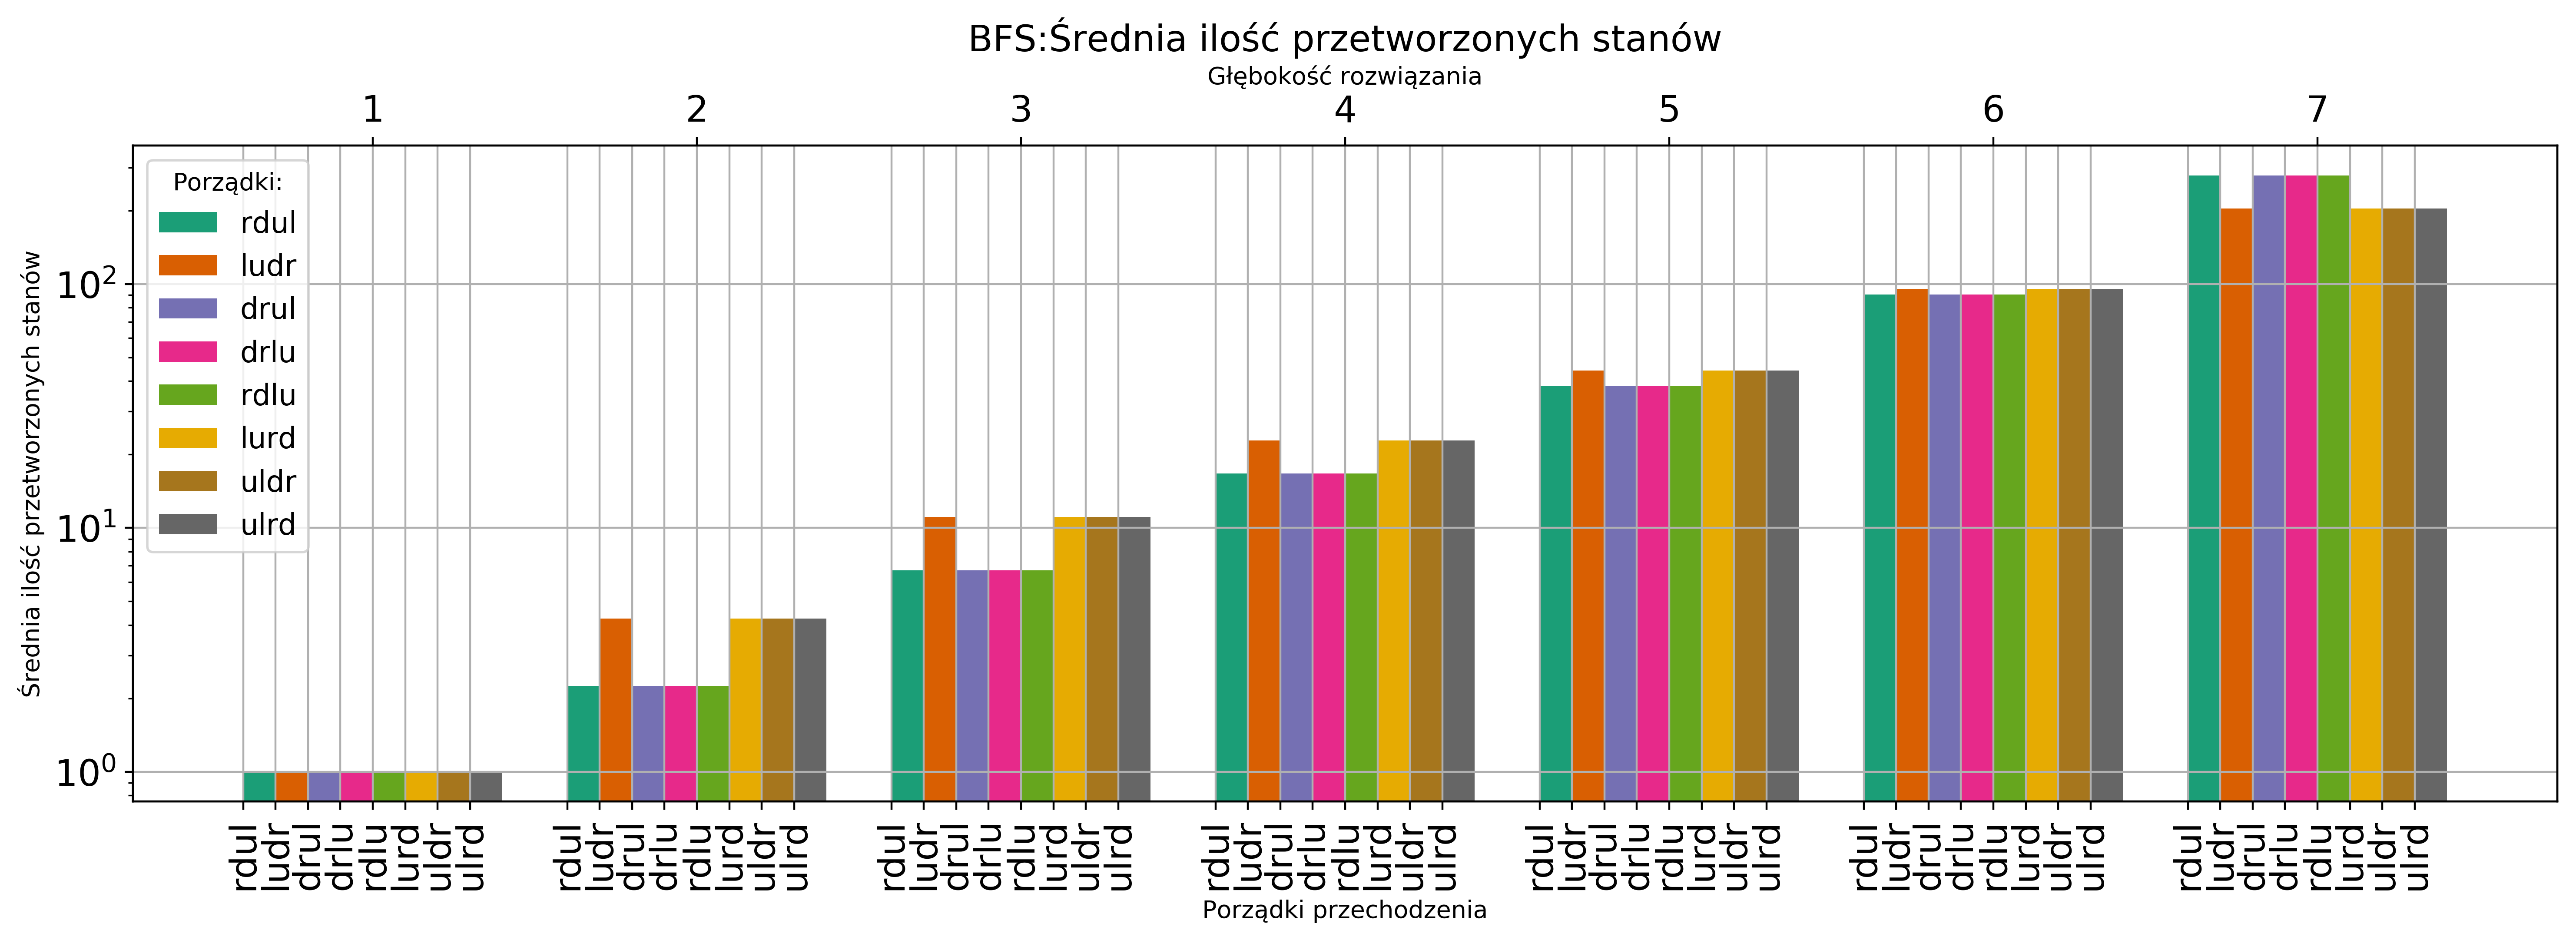
\includegraphics[width=\textwidth]{charts/BFS_processed.png}
    \caption{BFS -- Średnia ilość przetworzonych stanów}
    \label{BFS:processed}
    \vspace{0.2cm}
    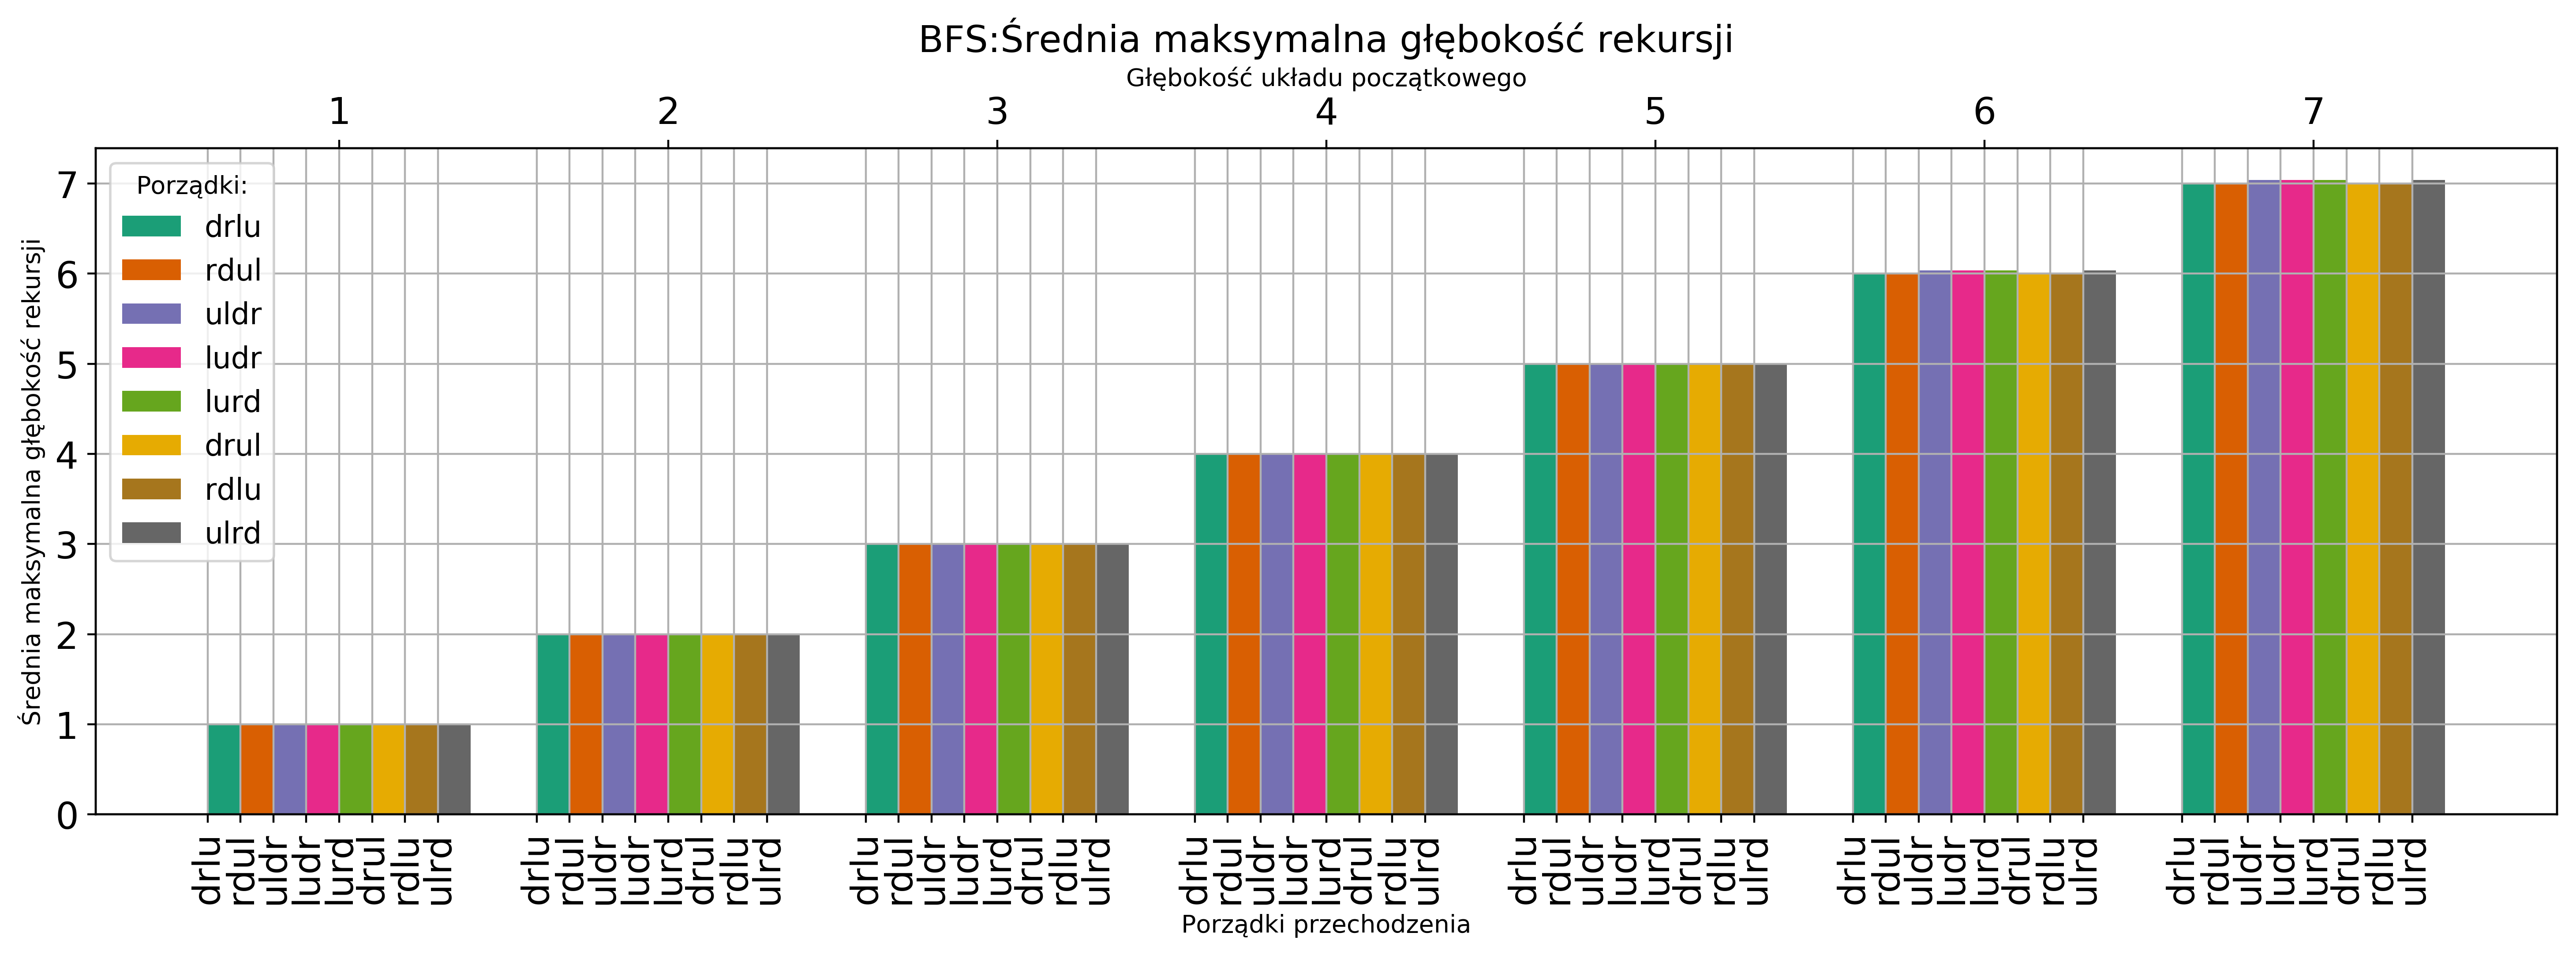
\includegraphics[width=\textwidth]{charts/BFS_recursed.png}
    \caption{BFS --  Średnia maksymalna głębokość rekursji}
    \label{BFS:time}

\end{figure}

\begin{figure}[H]
    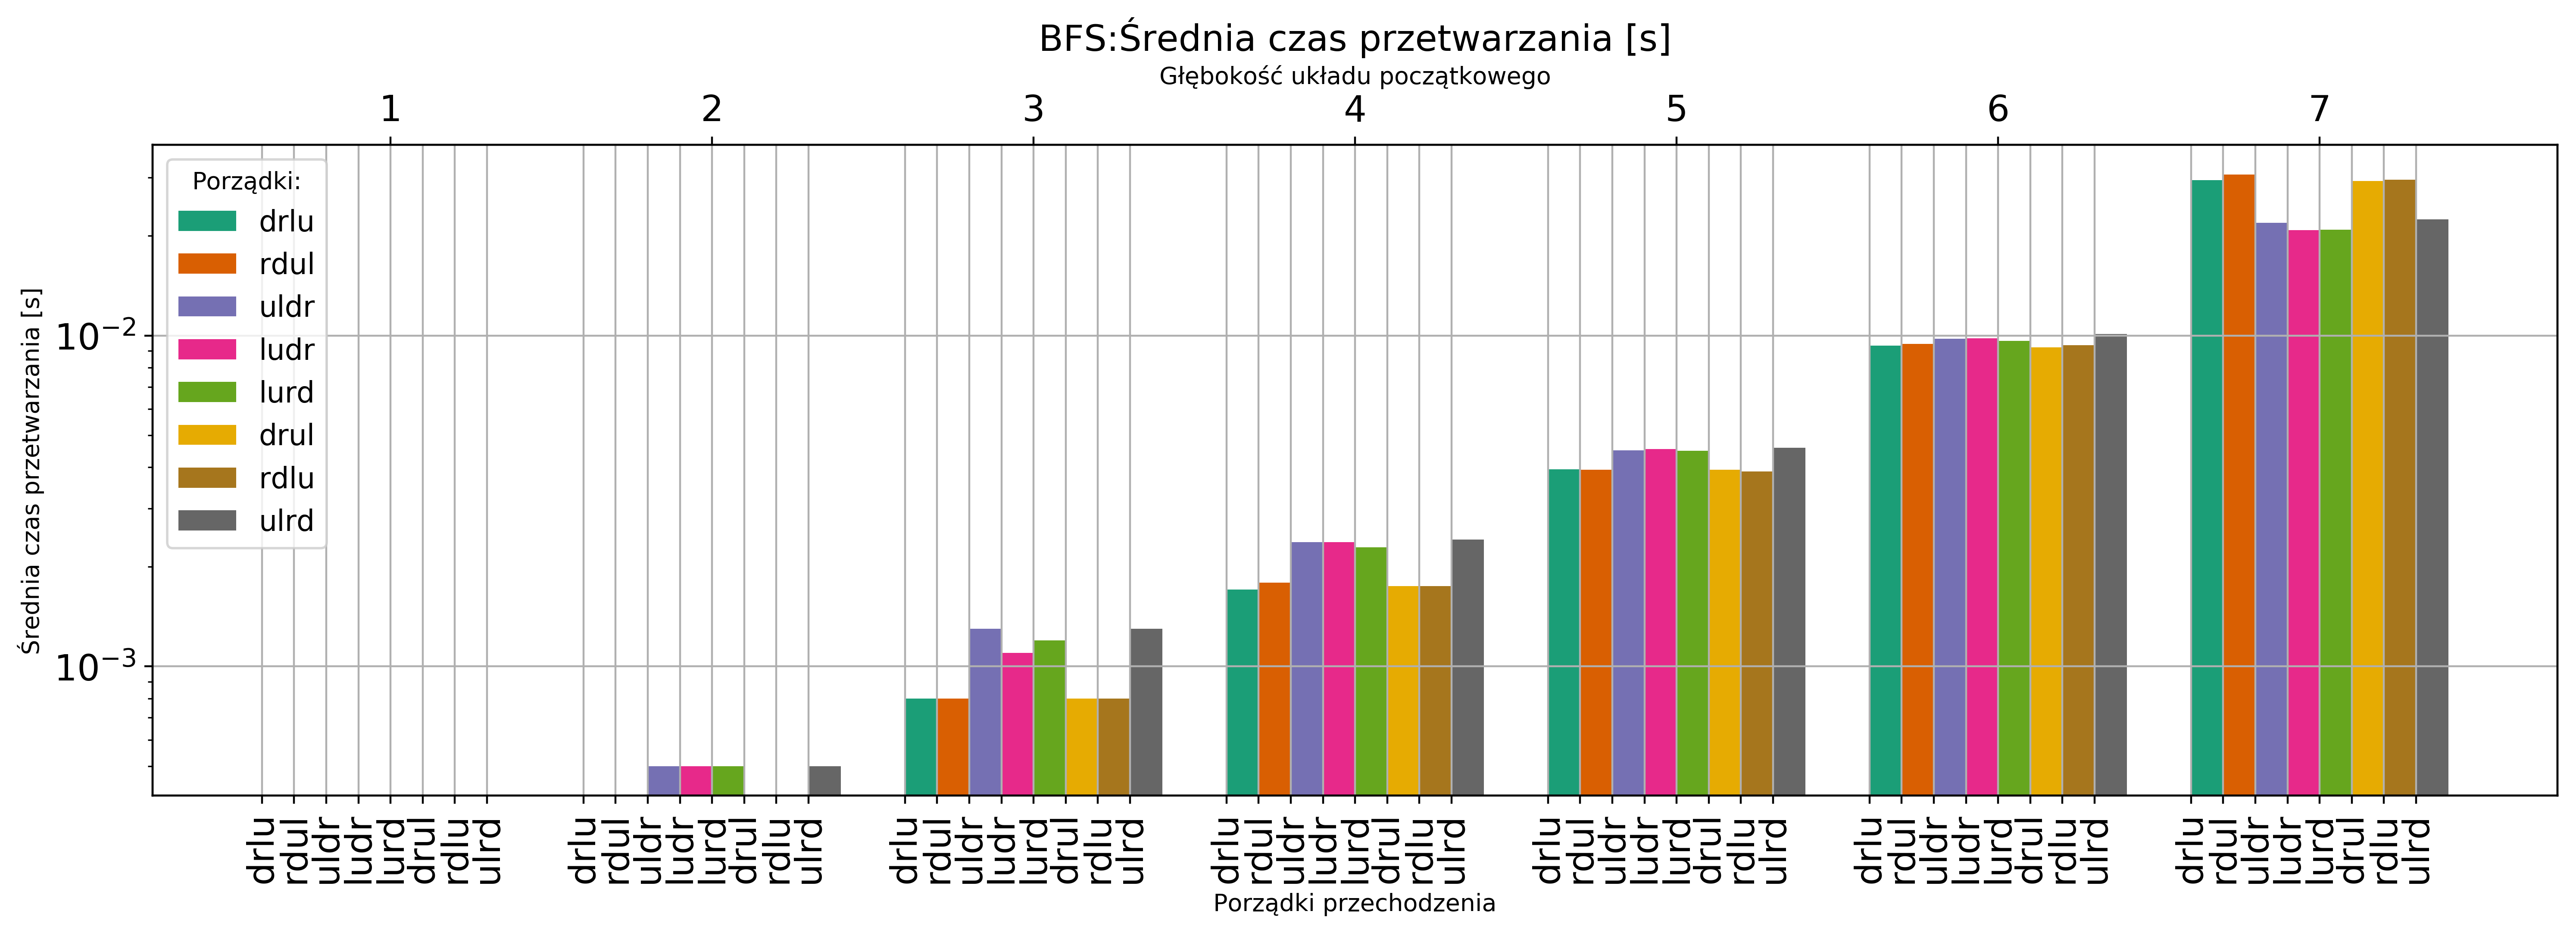
\includegraphics[width=\textwidth]{charts/BFS_time.png}
    \caption{BFS -- Średni czas przetwarzania}
    \label{BFS:time}
    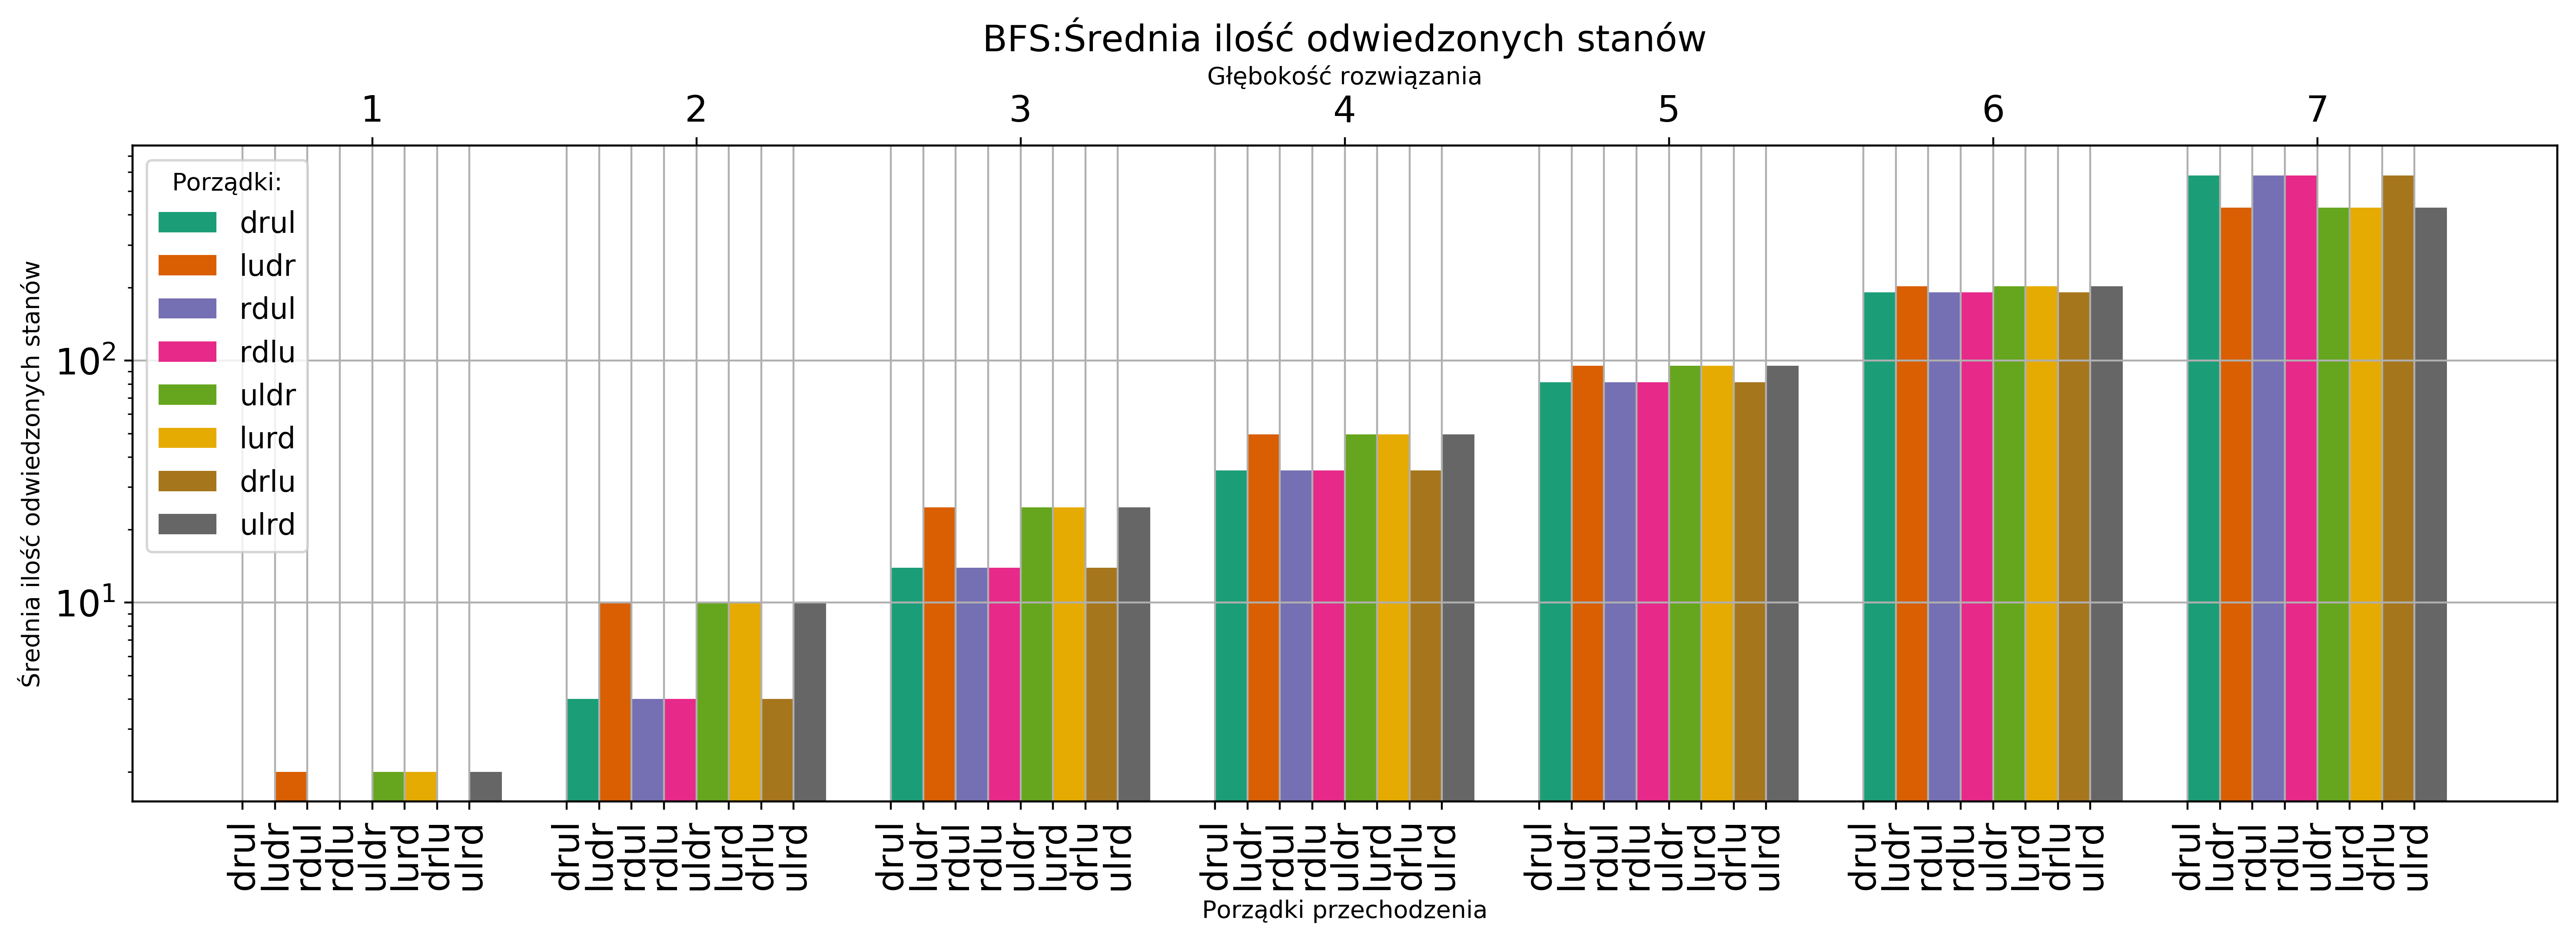
\includegraphics[width=\textwidth]{charts/BFS_visited.png}
    \caption{BFS -- ŚŚrednia ilość odwiedzonych stanów}
    \label{BFS:time}
\end{figure}

\begin{figure}[H]
    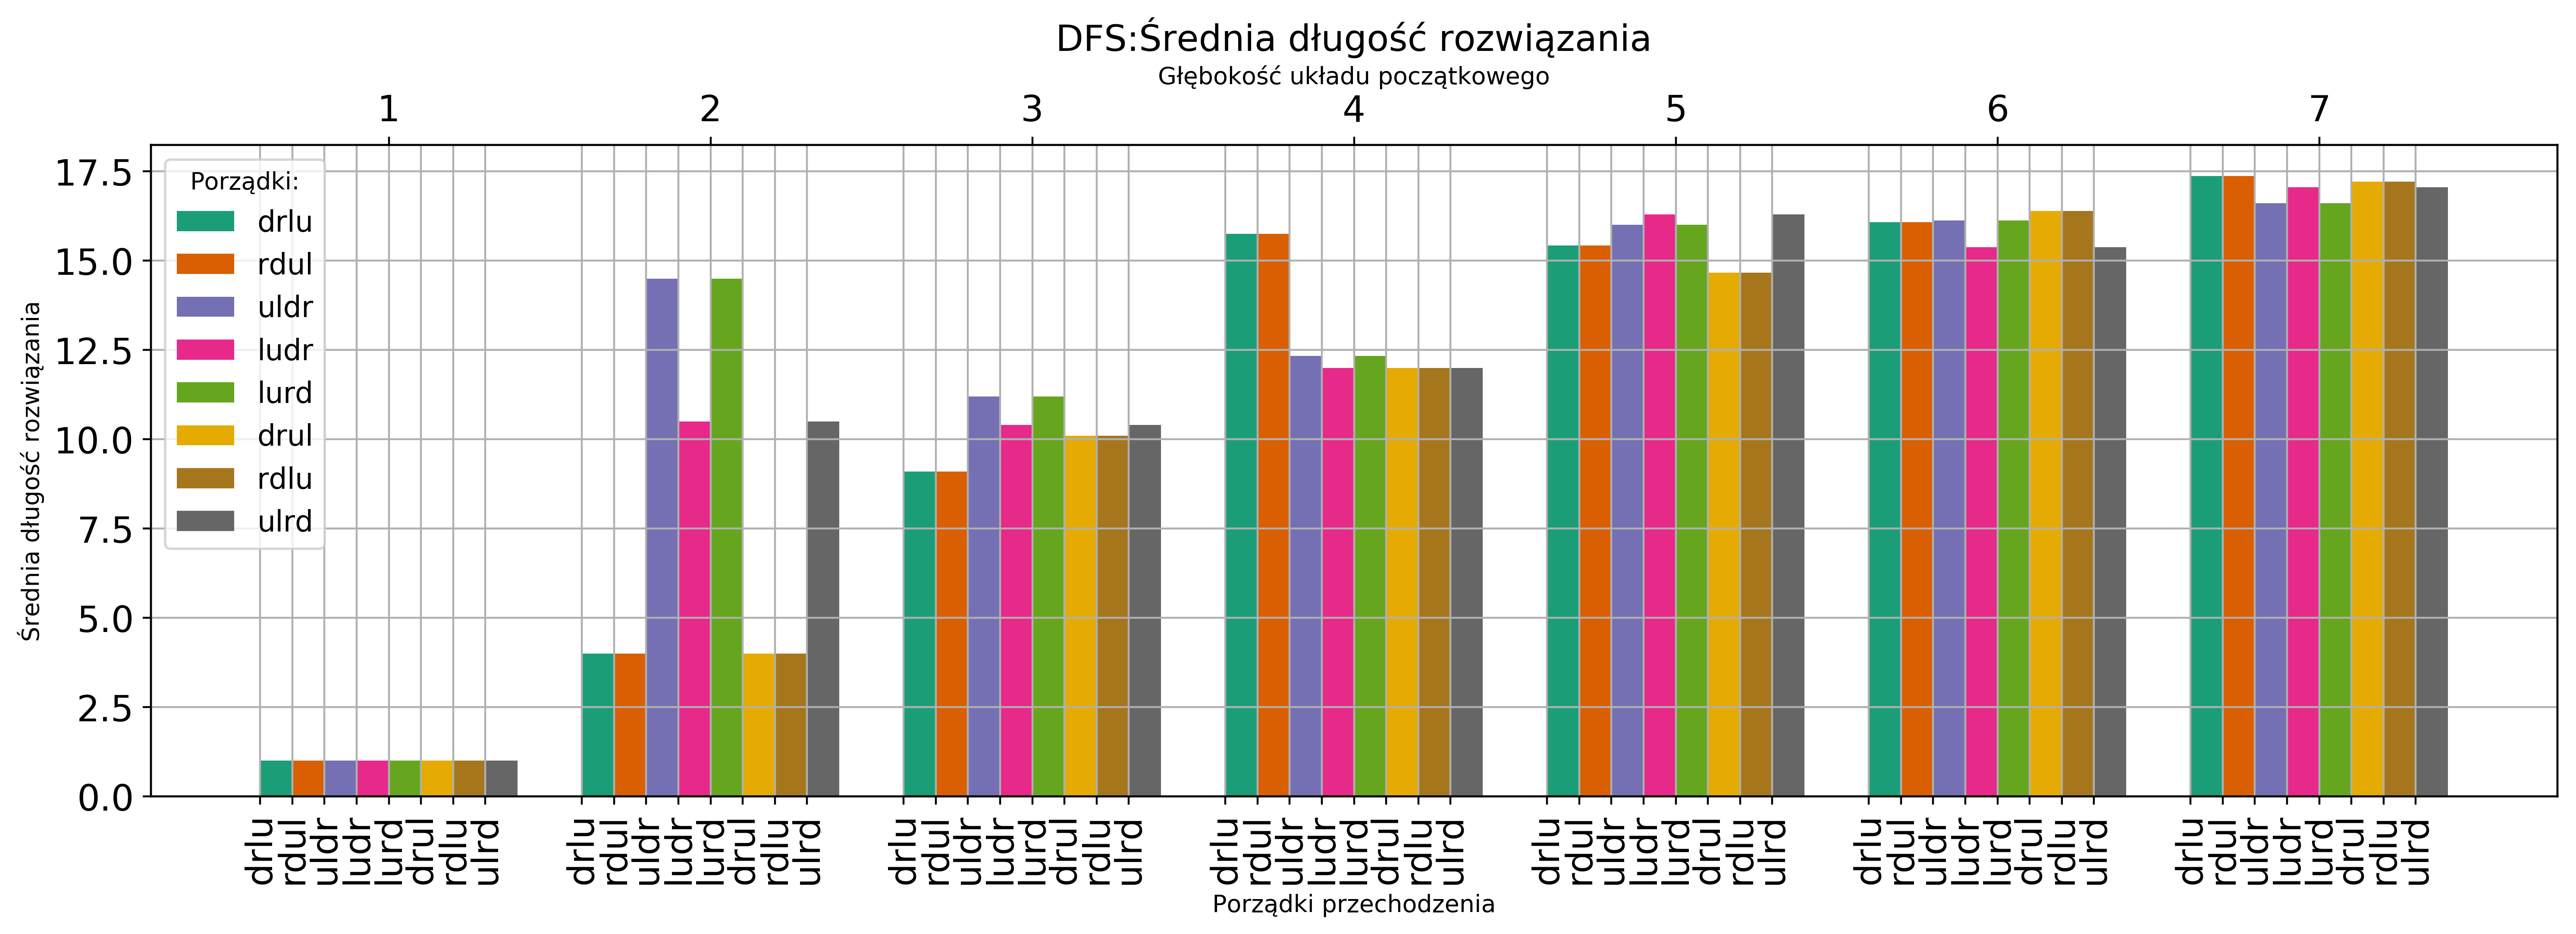
\includegraphics[width=\textwidth]{charts/DFS_path_length.png}
    \caption{DFS -- Średnia długość rozwiązania}
    \label{DFS:path_length}
    \vspace{0.2cm}
    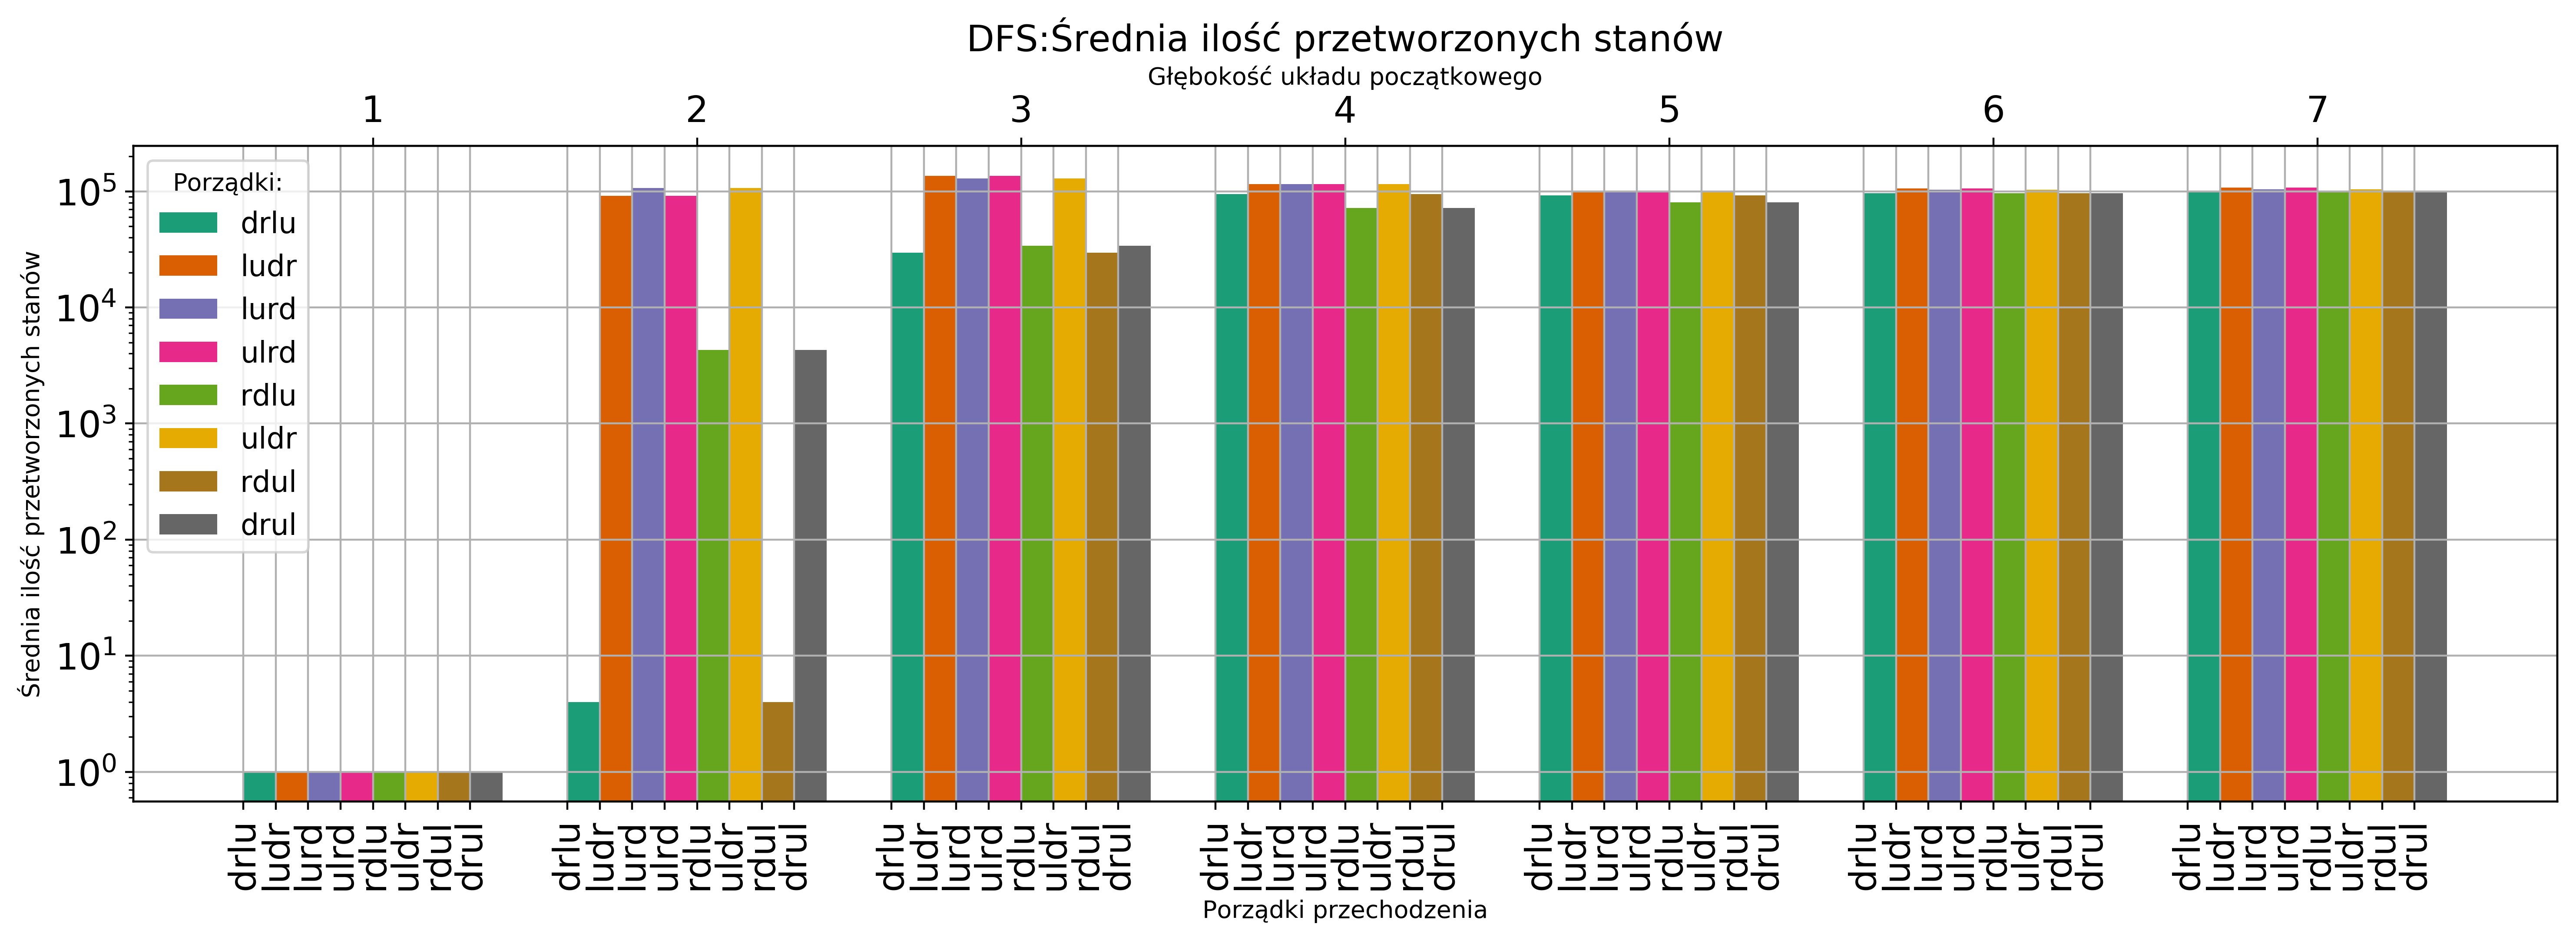
\includegraphics[width=\textwidth]{charts/DFS_processed.png}
    \caption{DFS -- Średnia ilość przetworzonych stanów}
    \label{DFS:processed}
    \vspace{0.2cm}
    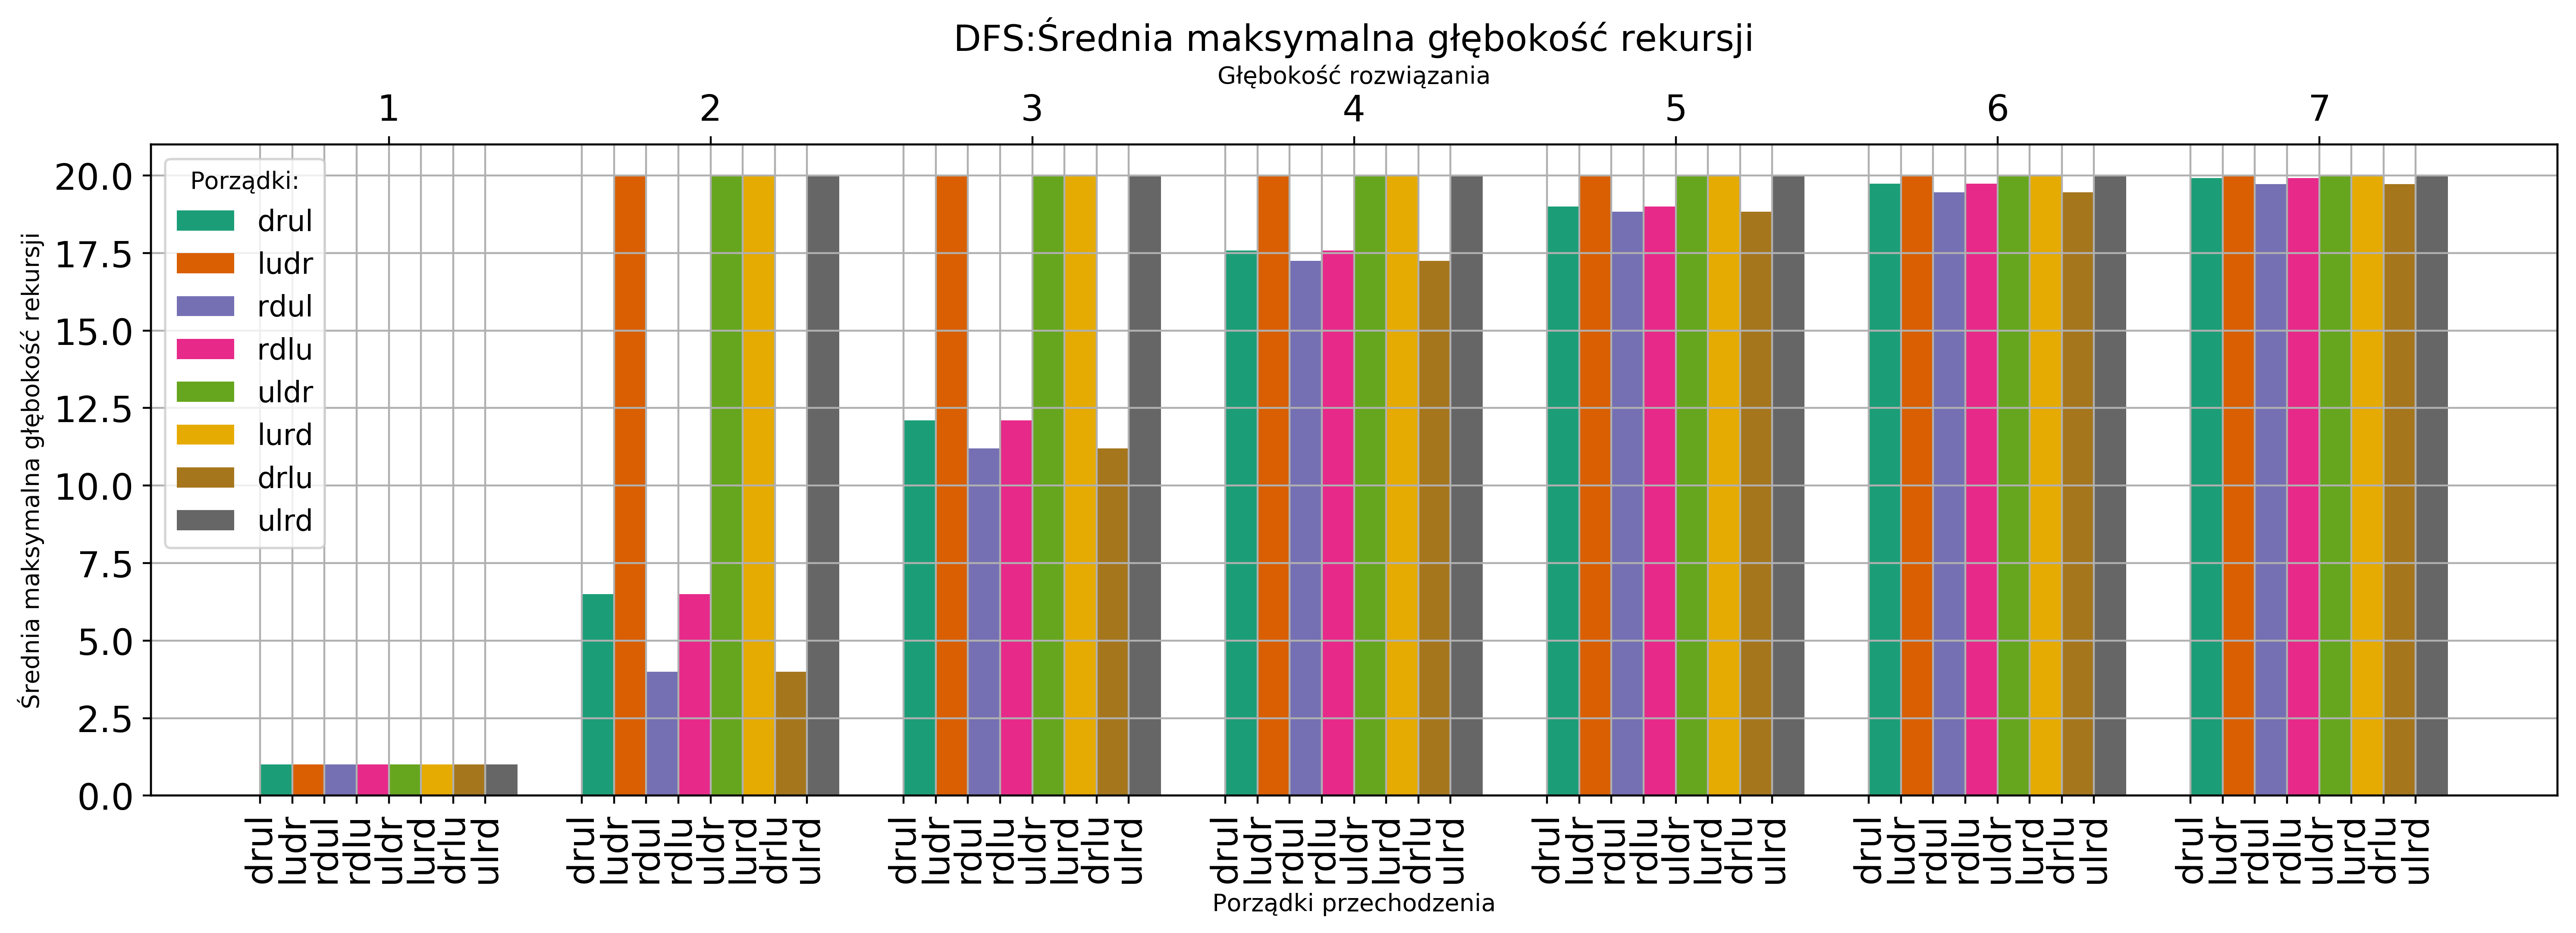
\includegraphics[width=\textwidth]{charts/DFS_recursed.png}
    \caption{DFS --  Średnia maksymalna głębokość rekursji}
    \label{DFS:time}

\end{figure}

\begin{figure}[H]
    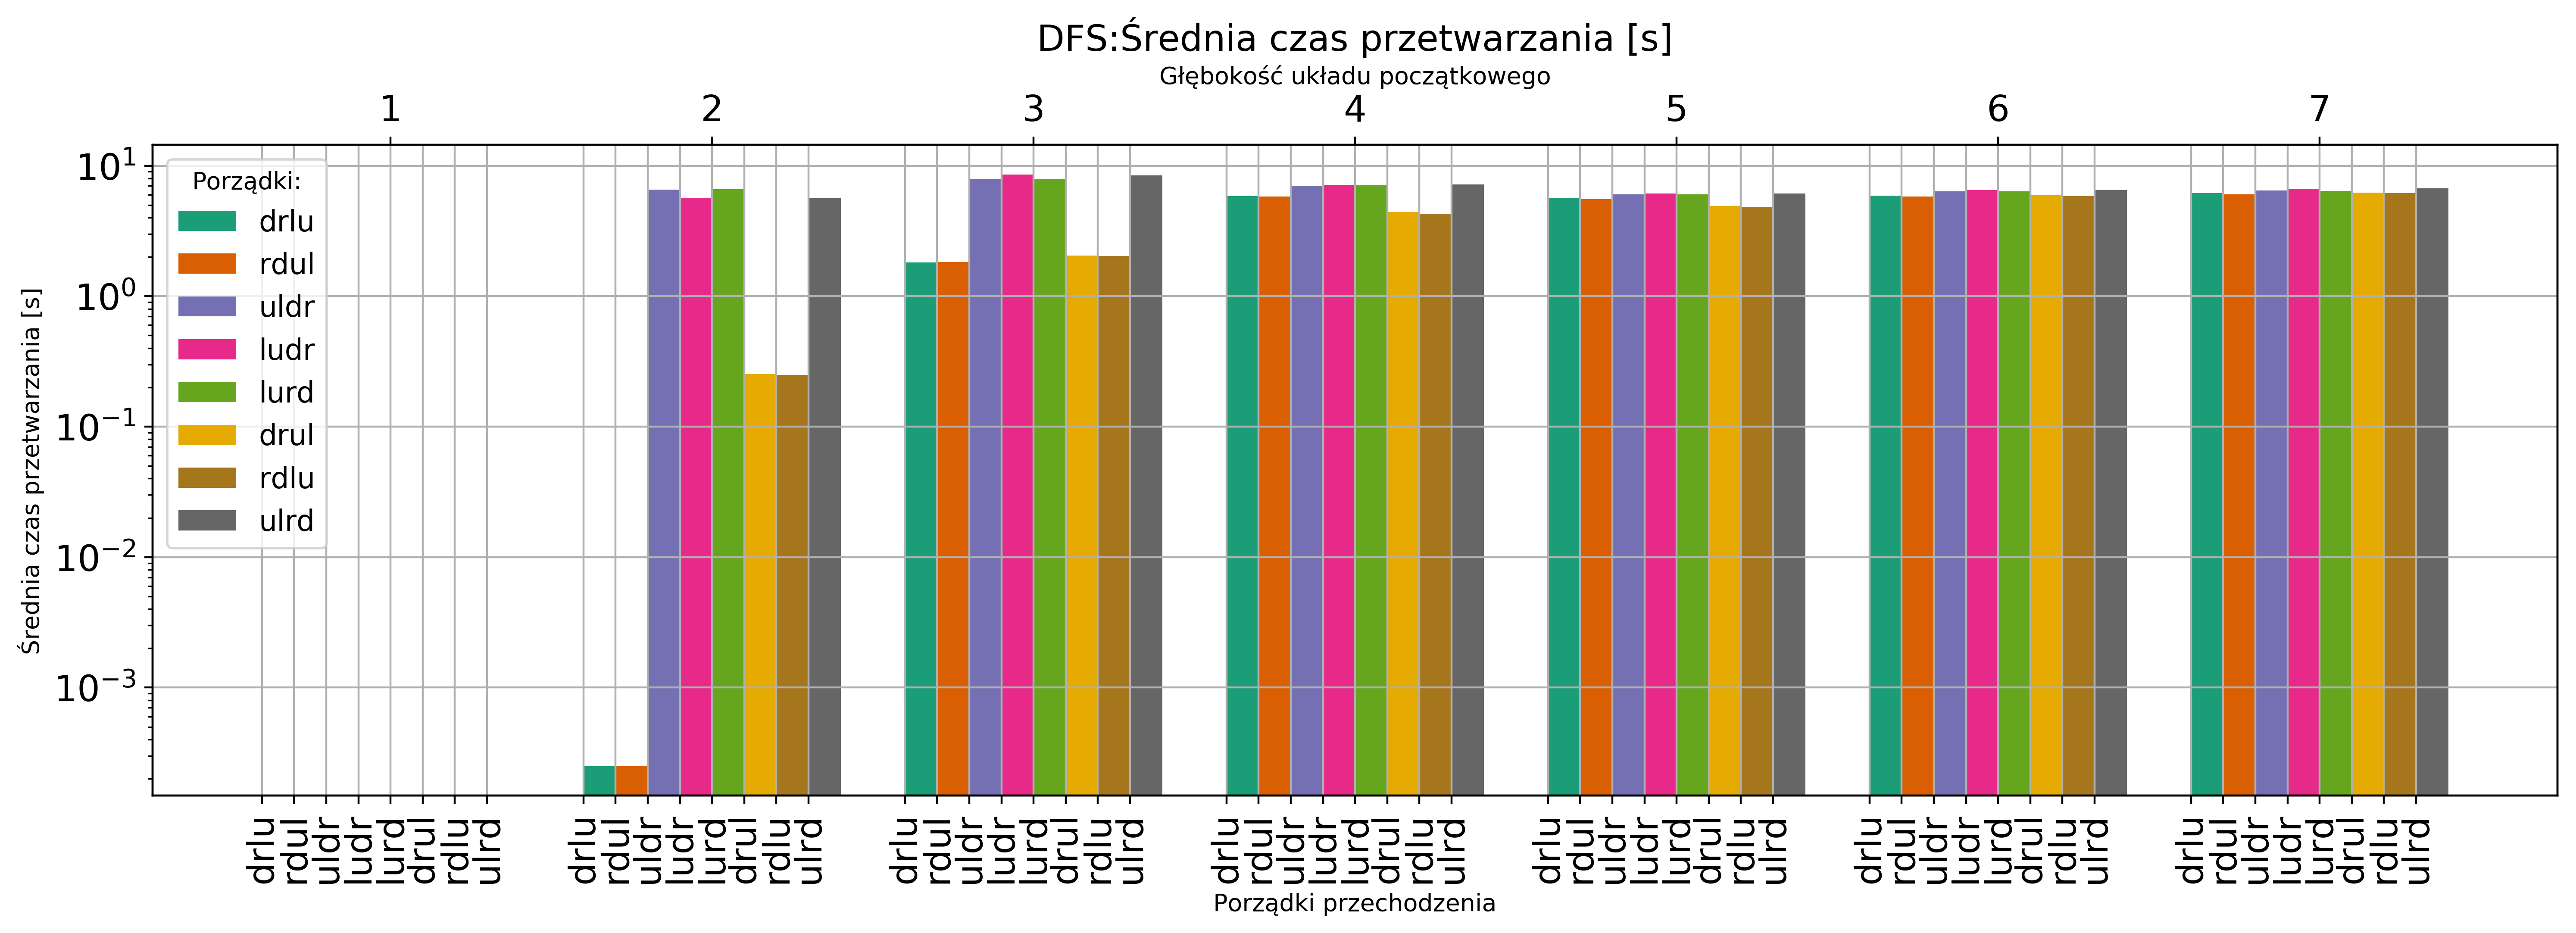
\includegraphics[width=\textwidth]{charts/DFS_time.png}
    \caption{DFS -- Średni czas przetwarzania}
    \label{DFS:time}
    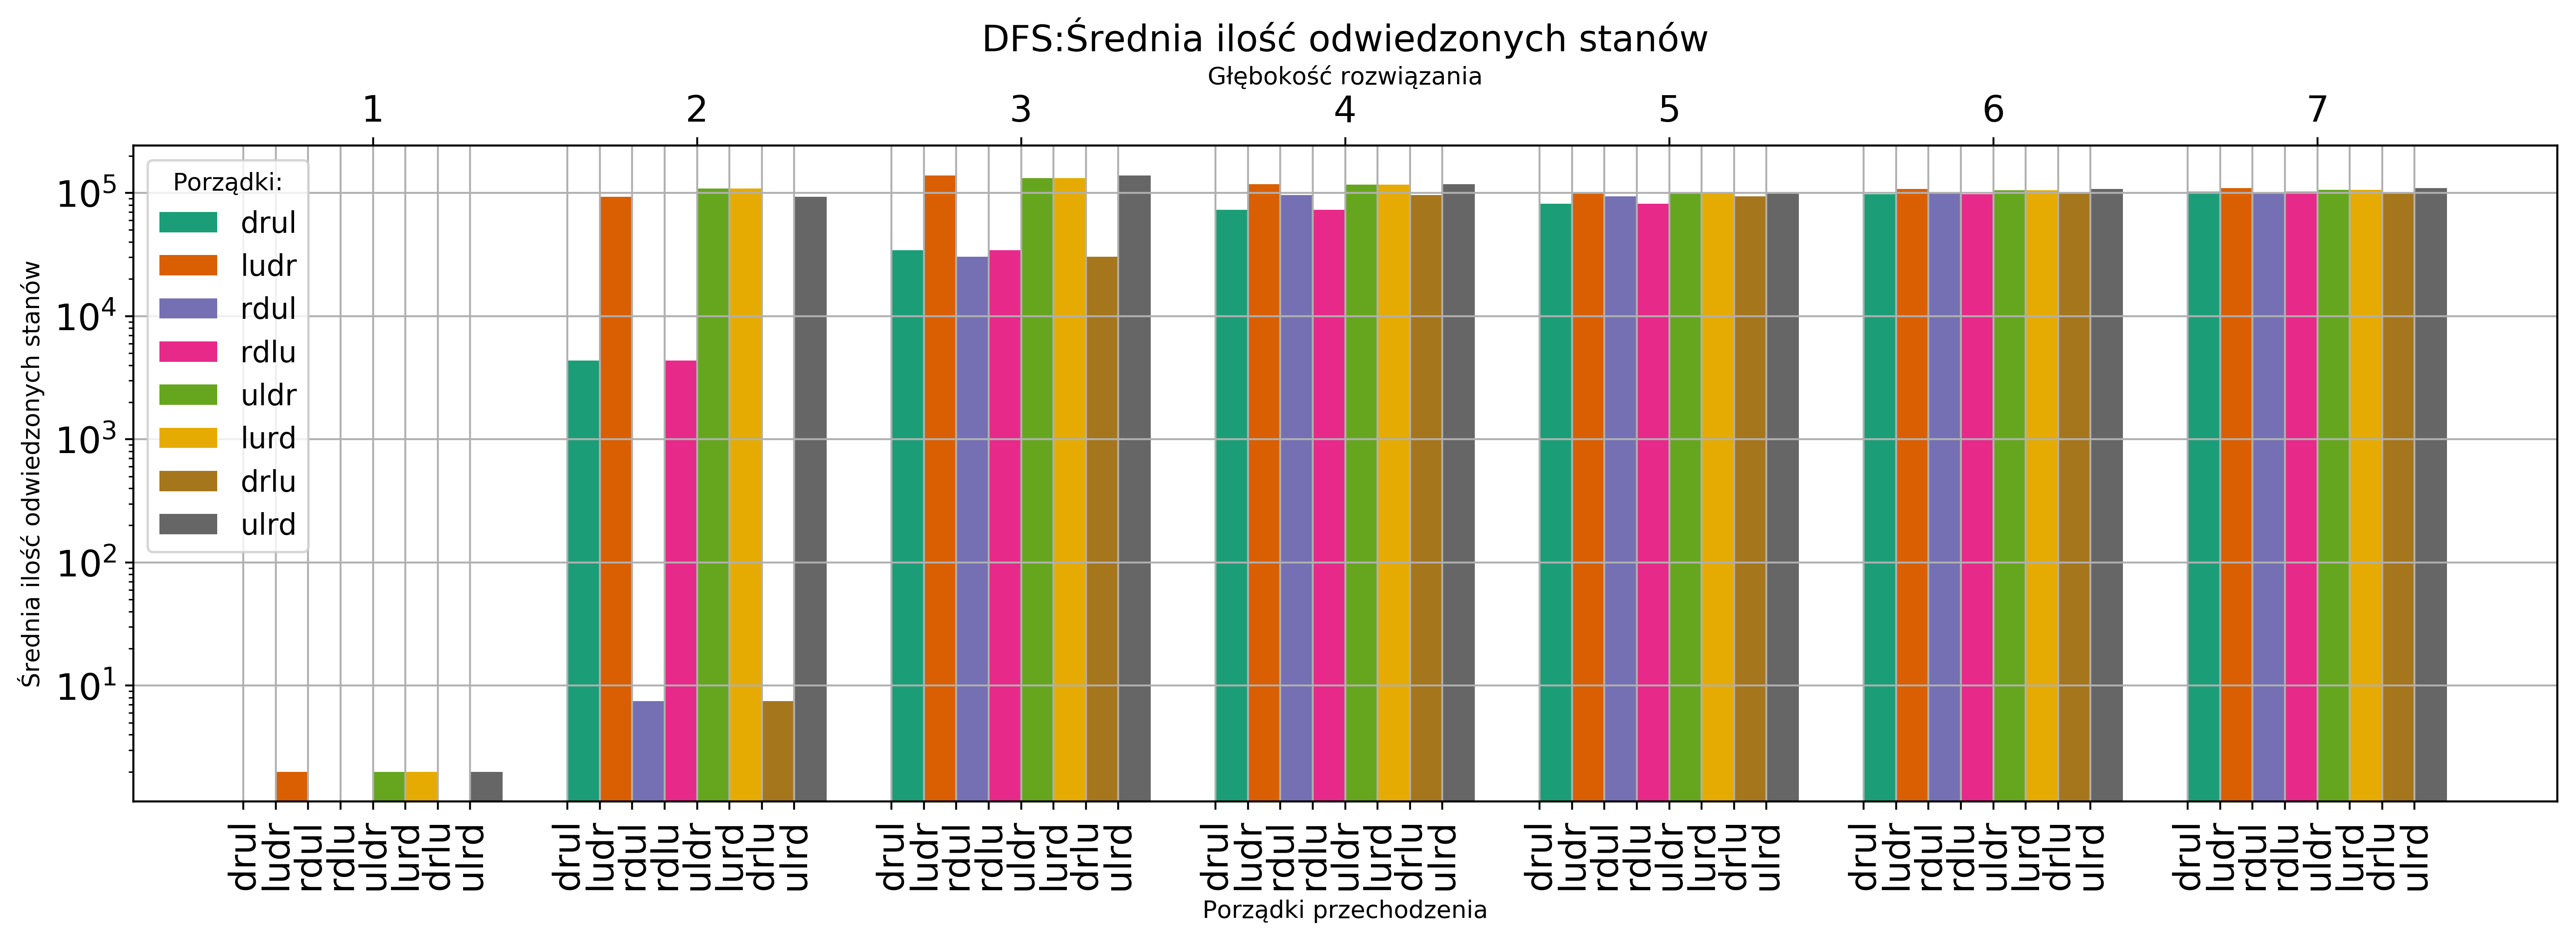
\includegraphics[width=\textwidth]{charts/DFS_visited.png}
    \caption{DFS -- ŚŚrednia ilość odwiedzonych stanów}
    \label{DFS:time}
\end{figure}



\restoregeometry

\section{Dyskusja}
{\color{blue}
Sekcja ta powinna zawierać dokładną interpretację uzyskanych wyników
eksperymentów wraz ze szczegółowymi wnioskami z nich płynącymi. Najcenniejsze
są, rzecz jasna, wnioski o charakterze uniwersalnym, które mogą być istotne
przy innych, podobnych zadaniach. Należy również omówić i wyjaśnić wszystkie
napotkane problemy (jeśli takie były). Każdy wniosek powinien mieć poparcie we
wcześniej przeprowadzonych eksperymentach (odwołania do konkretnych wyników).
Jest to jedna z najważniejszych sekcji tego sprawozdania, gdyż prezentuje
poziom zrozumienia badanego problemu.}

\section{Wnioski}
{\color{blue}
W tej, przedostatniej, sekcji należy zamieścić podsumowanie najważniejszych
wniosków z sekcji poprzedniej. Najlepiej jest je po prostu wypunktować. Znów,
tak jak poprzednio, najistotniejsze są wnioski o charakterze uniwersalnym.}

\begin{thebibliography}{0}
  \bibitem{l2short} T. Oetiker, H. Partl, I. Hyna, E. Schlegl.
    \textsl{Nie za krótkie wprowadzenie do systemu \LaTeX2e}, 2007, dostępny
    online.
\end{thebibliography}

{\color{blue}
Na końcu należy obowiązkowo podać cytowaną w sprawozdaniu literaturę, z której
grupa korzystała w trakcie prac nad zadaniem.}

\end{document}
